\documentclass[10pt, a4paper]{article}
\usepackage[utf8]{inputenc}
\usepackage[T1]{fontenc,url}
\usepackage{multicol}
\usepackage{multirow}
\usepackage{parskip}
\usepackage{lmodern}
\usepackage{microtype}
\usepackage{verbatim}
\usepackage{amsmath, amssymb}
\usepackage{tikz}
\usepackage{physics}
\usepackage{mathtools}
\usepackage{algorithm}
\usepackage{algpseudocode}
\usepackage{listings}
\usepackage{enumerate}
\usepackage{graphicx}
\usepackage{float}
\usepackage{hyperref}
\usepackage{tabularx}
\usepackage{siunitx}
\usepackage{fancyvrb}
%\usepackage{natbib}
%\bibliographystyle{dinat}
\usepackage[makeroom]{cancel}
\usepackage[margin=2.0cm]{geometry}
\usepackage{pdfpages}
\usepackage[margin=10pt, textfont={small, it}, labelfont={bf}, labelsep=endash]{caption}
\renewcommand{\baselinestretch}{1}
\renewcommand{\exp}{e^}
\renewcommand{\b}{\boldsymbol}
\newcommand{\h}{\hat}
\newcommand{\m}{\mathbb}
\newcommand{\half}{\frac{1}{2}}
\renewcommand{\exp}{e^}
\renewcommand{\bar}{\overline}
\setlength\parindent{0pt}


\begin{document}
\title{AST5220\\ Milestone II -- Recombination}
\author{
    \begin{tabular}{r l}
        Jonas Gahr Sturtzel Lunde & (\texttt{jonassl})
    \end{tabular}}
% \date{}    % if commented out, the date is set to the current date

\maketitle
Code found at \url{https://github.com/asdfbat/AST5220/tree/master/Project}
\vspace{0.7cm}

\section{Introduction}
Our main goal for this milestone is to model the optical depth $\tau$ and the visibility function $\tilde{g}$, as functions of the logarithmic scale factor, $x = \log{a}$. These parameters depend strongly on the free electron fraction $X_e$, which we will solve for using the Saha and Peebles equations for the regions of $X_e \geq 0.99$ and $X_e < 0.99$, respectively. Especially important for the evolution of the free electron fraction, and therefore also the optical depth and visibility function, is the period of recombination. Recombination was a rapid transition period around $370'000$ years after the Big Bang where the universe went from a ionized plasma soup, to consisting of neutral hydrogen as electrons and protons bound together.

The calculations will be performed under the assumption that the universe contains no heavier elements than Hydrogen ($Y_p = 0$). We will also be ignoring the event of \textit{reionization}, where the universe became ionized again around $x\approx -2$.

We also wish to pinpoint exactly at what times the events of recombination and last scattering happened. Recombination is more of a period characterized by sharp fall in the free electron fraction than it is a specific event, but we will define it as the point where $X_e = 0.5$. The surface of last scattering is the point in time where most of the photons we observe today would have last scattered, and corresponds to the point where the visibility function reaches its maximum value.


\section{Theory and method}
\subsection{The visibility function}
Our main goal is to model the visibility function $\tilde{g}(x)$ from the early universe until today, with special focus on the epoch of recombination. The visibility function is a probability function, representing the probability of any photon (as of today) to last have scattered at time $x$. If you asked random photons arriving from space when they last met a stranger, their answers would follow the distribution $\tilde{g}(x)$. It is an explicit function of the optical depth $\tau$ and its derivative, as
\begin{equation}\label{eqn:g_tilde}
    \tilde{g}(x) = -\tau^{\prime} e^{-\tau}
\end{equation}
Where the notation $\tau^\prime = \dv{\tau}{x}$ will be used throughout the report.

Being a probability function, it's normalized to one, as can be observed from integrating \ref{eqn:g_tilde}.
\begin{equation}
    \int_{-\infty}^{0} \tilde{g}(x) d x = 1
\end{equation}


\subsection{The optical depth}
The visibility function requires a solution of the optical depth $\tau(x)$. The optical depth represents the optical thickness the universe exhibits for photons originating at some time $x$. A high optical depth means photons travel very short distances before being absorbed or scattered. The optical depth can be related to the observed intensity of some source $I_0$ originating at a time/distance $x$, where we would observe an intensity today as $I = I_0\exp{-\tau(x)}$.

$\tau$ can be written as a differential equation on the form
\begin{equation}\label{eqn:tau_ODE}
    \tau^\prime = - c \sigma_T\frac{n_{e}(x)}{H(x)}
\end{equation}
where $c$ is the speed of light, $\sigma_T = \frac{8 \pi}{3} \frac{\alpha^{2} \hbar^{2}}{m_{e}^{2} c^{2}}$ is the Thompson scattering cross-section, $n_e(x)$ is the electron density, and $H(x)$ is the Hubble parameter. As we can see, the chase continues, and $\tau$ is dependent on the solution of both $n_e(x)$ and $H(x)$. An accounting of the solution of $H(x)$ can be found in Milestone I (\cite{Milestone1}), while $n_e(x)$ will be discussed in the coming sections.


\subsection{Dimensionality analysis}
Due to their fondness of confusing notation and immense pleasure in dropping terms from equations\footnote{Theories that this stems from laziness have been thoroughly debunked.}, astrophysicists often employ so-called natural units. This involves choosing a set of physical units such that a lot of commonly used constants become unity. For our purposes, this involves $c = \hbar = k_B = 1$. For this reason, equation like \ref{eqn:tau_ODE} might be found in the literature as
\begin{equation*}
    \tau^\prime = - \sigma_T\frac{n_{e}(x)}{H(x)}
\end{equation*}
with the factor of $c$ lacking. This might be awfully convenient during derivations, but when we at the end of the day require physical quantities in known units, we need a way of reintroducing these missing constants in a consistent way. This is known as dimensionality analysis, and entails looking at the apparent dimensions of the equation, comparing it to the dimensions it \textit{should} have, and inserting constants to make it so. For instance, we can easily see that the RHS of the equation above lacks units corresponding to those of the constant $c$, from the knowledge that $\tau'$ is unitless, and the RHS must therefore be so as well.

Appendix \ref{sec:appendixA} offers a walkthrough of the dimensional analysis required to reconstruct both the Saha and Peebles equation from their natural-unit forms.


\subsection{Free electron fraction and the Boltzmann equation}
The most important quantity deciding the optical depth is the free electron density $n_e$, or a very related quantity - the free electron fraction $X_e = \frac{n_e}{n_b}$, where $n_b$ is the baryon density (remember that we assume no heavier elements than Hydrogen). Under the same assumption, we know the baryon density of the universe to be $n_b = \frac{\Omega_{b,0}\rho_{c,0}}{m_ha^3}$ (see \cite{Milestone1}).

The density of any particle species in the universe can be modeled using the Boltzmann equation, presented below on its most general form.
\begin{equation*}
    \dv{f}{t} = C[f]
\end{equation*}
Here $f(t, \vec{x}, \vec{p})$ is the distribution function of the species in phase space, and the RHS contains all interactions with other species. During recombination, the interactions of interest taking place is electrons and photons recombining to form hydrogen, releasing a photon, and a photon knocking the electron loose from a hydrogen atom (Compton scattering). In other words, the allowed interactions are $e^- + p \leftrightarrow H + \gamma$. The Boltzmann equation applied to this interaction results in a ODE known as the Peebles equation, presented in section \ref{sec:Peebles}. 

The Peebles equation is numerically unstable at very early times ($X_e \approx 1$), among other reasons because one of the terms contain a $1-X_e$ term in the divisor. For the earliest intervals, we'll therefore instead employ the Saha equation.


\subsection{The Saha equation}
The Saha equation is an approximation of the Boltzmann/Peebles equation for $X_e \approx 1$. It is build upon the \textit{Saha approximation}, which reads that
\begin{equation*}
    \frac{n_e n_p}{n_H} \approx \qty(\frac{n_e n_p}{n_H})_{eq}
\end{equation*}
In other words, the system is very close to equilibrium, which holds for $X_e\approx 1$. The derivation of the natural-units Saha equation can be found in \cite[p. 70]{ModernCosmology2003}, and the dimensional analysis required to get it in full fledged form is shown in appendix \ref{sec:appendixA}. The full equation reads

\begin{equation}\label{eqn:Saha}
    \frac{X_{e}^{2}}{1-X_{e}} = A\ , \quad A = \frac{1}{n_{b}\hbar^3}\qty(\frac{m_{e} k_B T_{b}}{2 \pi})^{3 / 2} e^{-\epsilon_{0} / k_B T_{b}}
\end{equation}

\subsubsection{Solving the Saha equation}
The Saha equation \ref{eqn:Saha} is analytically solvable. Multiplying by $(1-X_e)$ on both sides and reshuffling gives us
\begin{equation*}
    \frac{X_e^2}{(1-X_e)} = A \quad \Rightarrow \quad X_e^2 + AX_e - A = 0
\end{equation*}
which is simply a second order equation in $X_e$, with solutions
\begin{equation*}
    X_e = - \frac{A}{2} \pm \frac{1}{2}\qty(A^2 + 4A)^{1/2}
\end{equation*}
The free electron fraction can't physically be negative. The positive solution reads
\begin{equation}\label{eqn:Saha_sol}
    X_e = - \frac{A}{2} + \frac{A}{2}\qty(1 + \frac{4}{A})^{1/2}
\end{equation}

We can also observe from \ref{eqn:Saha} that, as $X_e \rightarrow 1$, A will quickly converge towards zero as $A \propto X_e^2$. This will present a problem for equation \ref{eqn:Saha_sol}, as the $\frac{4}{A}$ term will diverge to infinity.

At the other end, as $X_e \rightarrow 1$, A will diverge to infinity, as $A \propto (1 - X_e)^{-1}$, likely to cause numerical inaccuracies.

A reasonable solution \cite{Grandma} to both these problems is to simply define
\begin{equation}\label{eqn:Saha_sol2}
    X_e =
    \begin{cases}
        \quad\quad 0& \quad A < 10^{-20} \\
        \quad\quad 1& \quad A > 10^6 \\
        - \frac{A}{2} + \frac{A}{2}\qty(1 + \frac{4}{A})^{1/2}& \quad else
     \end{cases}    
\end{equation}
avoiding any numerical stability issues without meaningful loss in precision.


\subsection{The Peebles equation}\label{sec:Peebles}
After the Saha regime ends, the solutions will be treated with the full Peebles equation. The equation can be found on its natural-unit form in \cite[p. 71]{ModernCosmology2003} as
\begin{equation}
    \label{eqn:Peebles}
    \dv{X_{e}}{x}=\frac{C_{r}\qty(T_{b})}{H}\qty[\beta\qty(T_{b})\qty(1-X_{e})-n_{H} \alpha^{(2)}\qty(T_{b}) X_{e}^{2}]
\end{equation}

The equation itself looks the same in natural units, but it contains a series of variables shown below, all of which have been rewritten with the proper dimensional analysis shown in appendix \ref{sec:appendixA}.
\begin{align}
    \label{eqn:1x}
    C_{r}\qty(T_{b}) &=\frac{\Lambda_{2 s \rightarrow 1 s}+\Lambda_{\alpha}}{\Lambda_{2 s \rightarrow 1 s}+\Lambda_{\alpha}+\beta^{(2)}\qty(T_{b})} \\
    \label{eqn:2x}
    \Lambda_{2 s \rightarrow 1 s} &=8.227 \mathrm{s}^{-1} \\
    \label{eqn:4x}
    \Lambda_{\alpha} &= H \frac{\qty(3 \epsilon_{0})^{3}}{(8 \pi)^{2} (c\hbar)^3 n_{1 s}} \\
    \label{eqn:5x}
    n_{1 s} &=\qty(1-X_{e}) n_{H} \\
    \label{eqn:6x}
    \beta^{(2)}\qty(T_{b}) &=\beta\qty(T_{b}) e^{3 \epsilon_{0} / 4 k_B T_{b}} \\
    \label{eqn:7x}
    \beta\qty(T_{b}) &= \alpha^{(2)}\qty(T_{b}) \qty(\frac{m_{e} k_B T_{b}}{2 \pi \hbar^2})^{3 / 2} e^{-\epsilon_{0} / k_BT_{b}} \\
    \label{eqn:8x}
    \alpha^{(2)}\qty(T_{b}) &= \frac{8}{\sqrt{3 \pi}} \sigma_T c \sqrt{\frac{\epsilon_{0}}{k_B T_{b}}} \phi_{2}\qty(T_{b}), \quad \sigma_{T}=\frac{8 \pi}{3} \frac{\alpha^{2} \hbar^{2}}{m_{e}^{2} c^{2}} \\
    \label{eqn:9x}
    \phi_{2}\qty(T_{b}) &=0.448 \ln \qty(\epsilon_{0} / k_B T_{b})
\end{align}

The baryon temperature is non-trivial, but a good approximation \cite{Euler} is to assume that it evolves naturally with the photon temperature, such that
\begin{equation*}
    T_{b} = T_{CMB}a^{-1} = \SI{2.725}{K}\cdot a^{-1}
\end{equation*}


\section{Implementation}
\subsection{General Overview}
The code used in this report can be found at \url{https://github.com/asdfbat/AST5220/tree/master/Project}. The simulations themselves are found in the \texttt{src/} directory, and is built upon the C++ code template provided by Hans Arnold Winther.

The code builds upon the work from Milestone I \cite{Milestone1} and the associated code, found in the \textit{Background cosmology} class in \texttt{src/BackgroundCosmology.cpp}.

The \textit{RecombinationHistory} class found in \texttt{src/RecombinationHistory.cpp} covers the work done in this milestone. The associated \texttt{Makefile} can be run as \textbf{make all run} to compile and run all code both from this milestone, and dependent code from Milestone I. This will produce data files \texttt{data/recombination.txt} and \texttt{data/recombination\_saha.txt}, which are analyzed in \texttt{Python/m2\_plotting.ipynb}.

\subsection{The electron number density solver}
The \textit{RecombinationHistory} class takes as constructor arguments an instance of the \textit{BackgroundCosmology} class, as well as the helium number fraction $Y_p$, which we are setting to zero. The \textit{solve} method calls first upon the method \textit{solve\_number\_density\_electrons}, which employs first the Saha equation solution \ref{eqn:Saha_sol2} for $X_e \leq 0.99$, and thereafter solves the Peebles equation for $X_e > 0.99$. The Peebles equation is solved as an ODE using the ODESolver class from the GSL library, which is wrapped in the helperclass \textit{ODESolver} found in \texttt{src/ODESolver.cpp}. The equations are solved in the interval $x\in [-20, 4]$ using $10^5$ linearly spaced points. The results of $X_e$ are splined using the spline class of the GSL library, again wrapped in a helperclass, \textit{Spline}, found in \texttt{src/Spline.cpp}. We in reality spline $\log{X_e}$, as it behaves more smoothly in $x$, and simply undo this whenever we need $X_e$.

\subsection{The optical depth solver}
With the solution of $X_e$ (and thereby $n_e$) known and splined, the \textit{solve} method calls upon the\\
\textit{solve\_for\_optical\_depth\_tau} method. This method solves \ref{eqn:tau_ODE} for $\tau(x)$ using the GSL ODESolver implementation over $x\in[-20, 0]$, using $10^5$ points. The only known value of $\tau$ is today, where $\tau(x=0) = 0$, while the initial condition at $\tau(x=-20)$ is not known. For this reason, we substitute $x \rightarrow -x$ in equation \ref{eqn:tau_ODE}, and solve it instead in the reversed interval $x\in[0, 20]$.\footnote{The negative substitution in $x$ means that this is in reality the interval $x\in [0, -20]$, but the ODESolver appears not to allow solving of ODEs with negative timesteps, so the substitution of $x$ is necessary.} Another possible solution is simply to set the initial condition $\tau(x=-20)$ to some arbitrary value, and simply rescale the final solution such by subtracting $\tau(x=0)$. The former solution was chosen because the latter suffer from numerical inaccuracies due to the span of values over many orders of magnitudes.

The solution of $\tau$ is splined, together with its first two derivatives with regards to $x$. The first derivative is known from the ODE, while the second is found using a built-in differentiator in the spline class.

The result of $\tau$ is used to calculate the visibility function $\tilde{g}$ from \ref{eqn:g_tilde}, which is also splined, together with its first two derivatives in $x$, both calculated using the spline differentiator.



\section{Results}
\subsection{Free electron fraction}
Figure \ref{fig:Xe} shows the evolution of the free electron fraction as function of $x$ for both the Saha approximation, and the full Peebles equation aAll solutions quoted as "using the Peebles equation" still employ the Saha before the "Saha limit" of $X_e < 0.99$). We can see that the solutions diverge shortly after the Saha limit, with the Saha solution quickly falling off towards zero, while the Peebles solution stabilizes towards a value of $X_e(x=0) = 1.9\times 10^{-4}$ today.

The flattening of the free electron fraction represents the freeze out of electrons, where they decouple from the thermal bath. The equilibrium solution of the system predicts an exponential suppression of the free electron fraction as the temperature drops, in line with the Saha equation. However, the process loses its efficiency due to the decaying interaction rate as the universe expands, and the freeze out occurs, giving the non-equilibrium value seen from the Peebles solution.

Saha also predicts an earlier point of recombination than Peebles does, at $x = -7.17$ instead of $x = - 7.23$. This is of course simply because it drops faster to the recombination definition of $X_e = 0.5$. The surface of last scattering is also indicated in the figures, which we'll come back to in section \ref{sec:results:g_tilde}.



\begin{figure}[H]
    \centering
    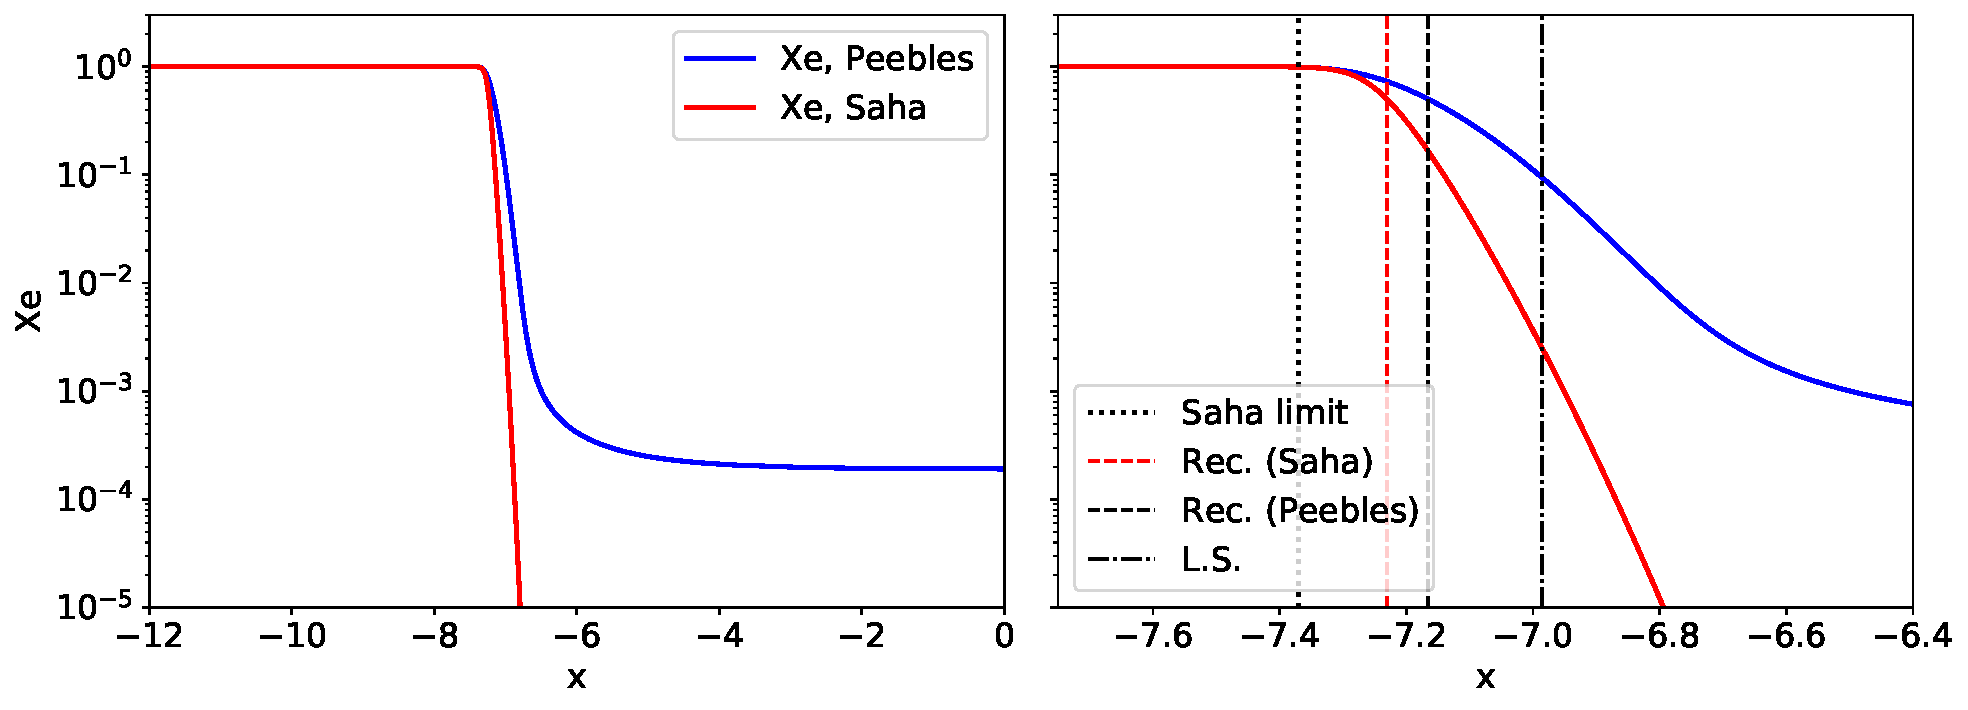
\includegraphics[scale=0.5]{../m2_figs/Xe.pdf}
    \caption{Figure showing the relative electron density as function of $x=\log{a}$, solved using the Saha equation only (red), and both the Saha and Peebles equation (blue), with a transition at $X_e = 0.99$. The right panel shows a zoomed in version, additionally showing the following events as vertical lines: 1) The Saha-Peebles transition limit, at $X_e = 0.99$. 2) The event of recombination, defined as $X_e = 0.5$, as calculated from the Saha equation only. 3) The event of recombination, as calculated by both the Saha and Peebles equation. 4) The surface of last scattering, defined as the point where $g$ reaches its maximum value (see figure \ref{fig:g_tilde}).}
    \label{fig:Xe}
\end{figure}


\subsection{Optical depth}
Figure \ref{fig:tau} shows the optical depth $\tau$ as function of $x$, as well as its derivatives in $x$. We see that $\tau(x)$ (apart from per definition falling to zero at $x=0$) exhibits three distinct regions. Looking forward in time from $x=-12$, we see that the early universe is incredibly optically thick. The mean free path was in this era very small, due to the dense plasma soup state the universe found itself in. The optical depth decreases "linearly"\footnote{since its log-plotted against $x$, linear behavior corresponds to exponential dependence on $x$, which again corresponds to power-law dependence in $a$} until around $x=-7.4$, where $X_e$ starts undergoing a sharp decline due to recombination. During this region, we see a sharp decline in the optical depth as the universe changes from a coupled soup state to one consisting almost entirely of neutral Hydrogen (as well as a decent fraction of Helium, which we won't consider). Half-way through this rapid drop, around $x=-6.9$, $\tau$ crosses the value of $1$, which is known as the surface of last scattering, and represents the \textit{most probable} point of origin for any photon observed today. As $X_e$ flattens out, $\tau$ again enters a new phase of less steep decline, before falling to zero today.

Looking back at equation \ref{eqn:tau_ODE}, we see that $-\tau'(x)$ is simply the ratio between what's called the \textit{scattering rate} $n_e\sigma_T$ \cite[p. 72]{ModernCosmology2003}, and the Hubble parameter $H(x)$. The Hubble parameter has the simple behavior of $H\propto \exp{-2x}$ for $x<-8.6$ and $H\propto \exp{-1.5x}$ for $x>-8.6$ (see \cite{Milestone1}), while the behavior of the free electron fraction can be seen in appendix \ref{sec:appendixC}. It's easy to see that the behavior of $-\tau(x)$ around the event of recombination very much corresponds to the behavior of $n_e(x)$ (or the scattering rate, if you wish, which is only different up to a constant).



\begin{figure}[H]
    \centering
    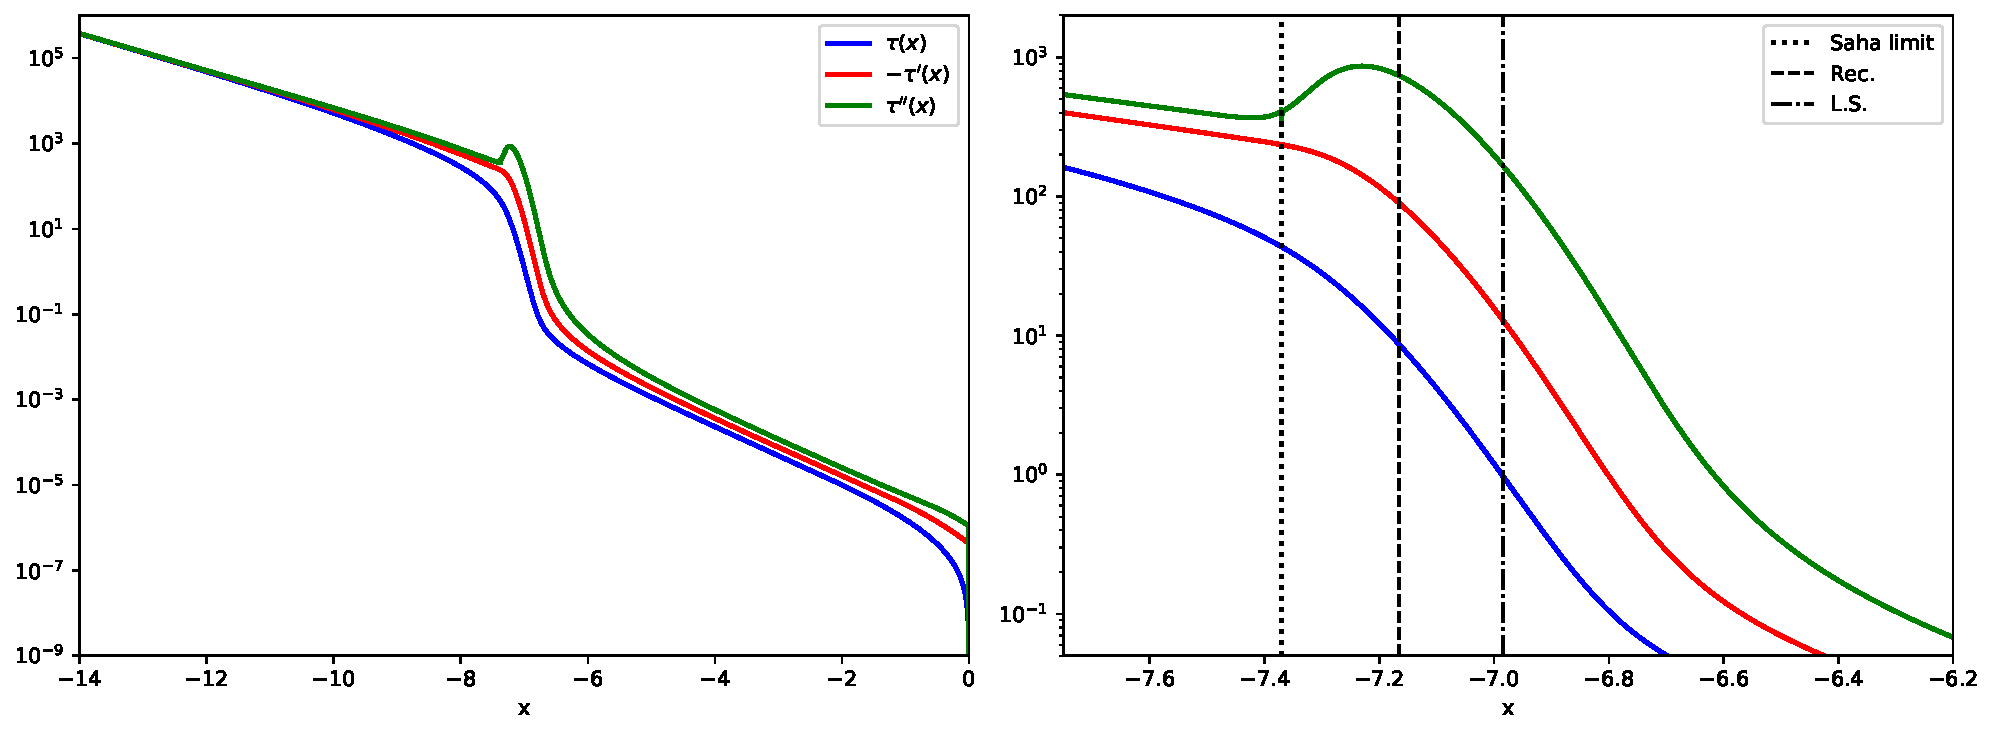
\includegraphics[scale=0.5]{../m2_figs/tau.pdf}
    \caption{Figure showing the optical depth $\tau(x)$, as well as its derivatives (with regards to $x$). The right panel shows a zoomed in version, in addition to vertical lines indicating events described in \ref{fig:Xe}.}
    \label{fig:tau}
\end{figure}


\subsection{Visibility function}\label{sec:results:g_tilde}
Figure \ref{fig:g_tilde} shows the visibility function $\tilde{g}$ and its derivatives as function of $x$. As previously stated, the visibility function is a probability distribution of when photons last scattered. As we can see, it is very strongly peaked around the event of last scattering (LS) at $x = -6.98$, this event being defined as the peak of $\tilde{g}$. The visibility function is very steeply sloped before LS, and somewhat slacker after the event. This means a photon is more likely to have scattered again somewhat after LS than it is to have passed through LS without scattering. Looking no further back than the event of recombination, at $x = -7.17$, the probability of having last scattered has fallen to virtually zero.

The strong peaking of the visibility function is important to us, as it means all the photons emitted (and observed today as the CMB) originated from the same time period, holding the blueprints to the fluctuations in the universe at one point in time very long ago.

The derivatives of $\tilde{g}$ are pretty self-explanatory, as the shape of $\tilde{g}$ is very simple (a somewhat skewed gaussian). The first derivative shows the asymmetry of $\tilde{g}$, as we can see it being much more strongly peaked before LS than after. The second derivative tells a similar story, having one positive peak at each side of LS, the first one being much more prominent, speaking to a steeper convex shape in $\tilde{g}$.


\begin{figure}[H]
    \centering
    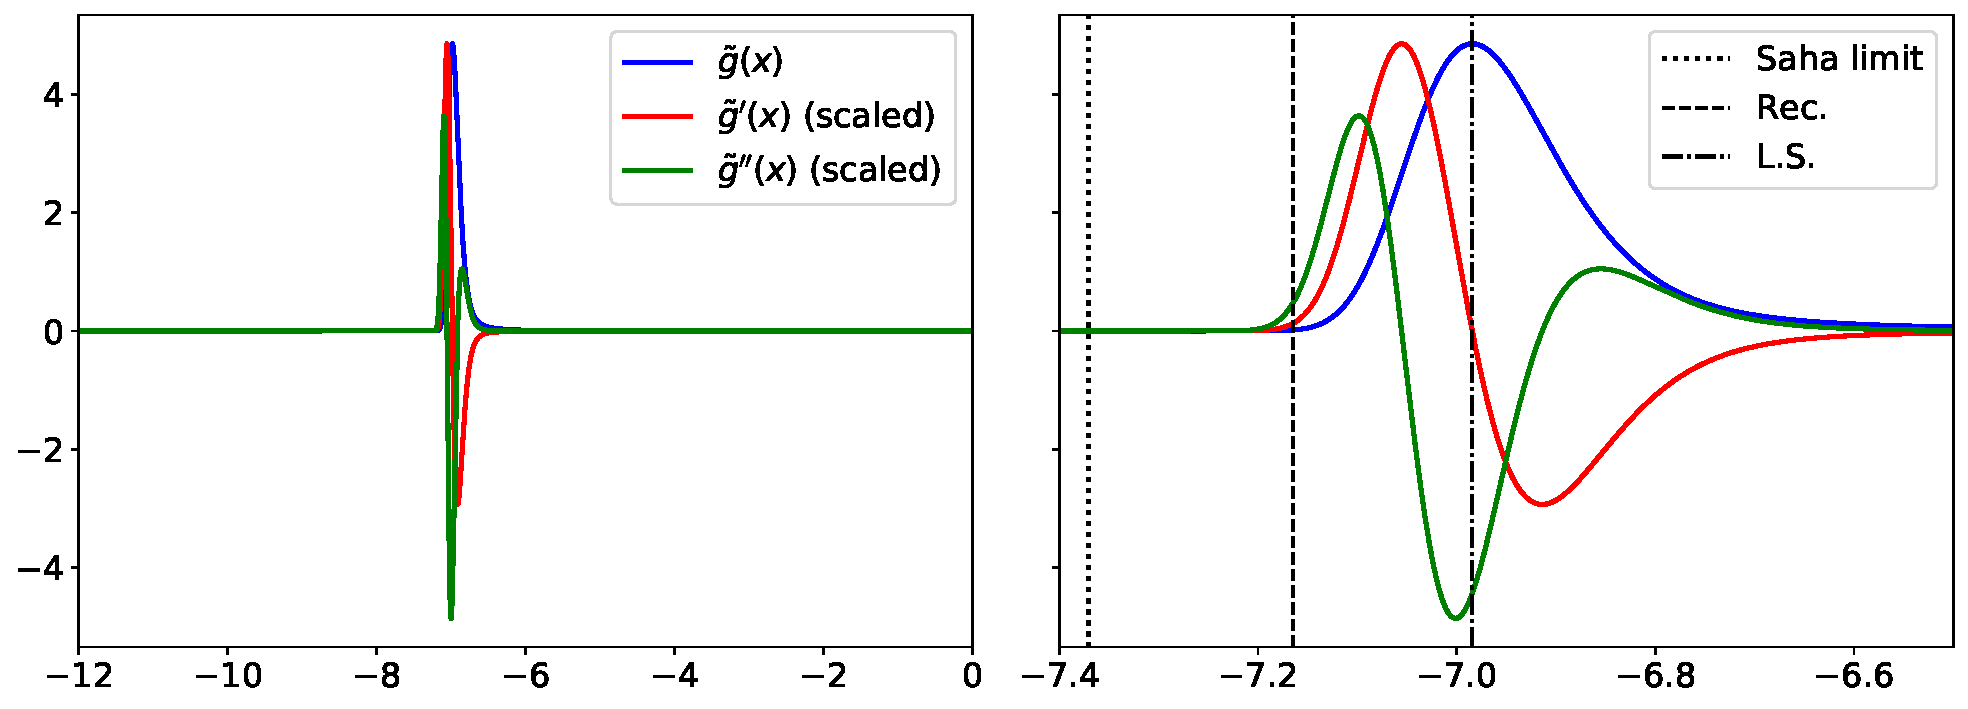
\includegraphics[scale=0.5]{../m2_figs/g_tilde.pdf}
    \caption{Figure showing the visibility function $\tilde{g}(x)$, and its derivatives (with regards to $x$). The first and second derivatives are scaled with factors of $0.0956$ and $0.0049$, respectively, such that their maxima coincide with that of $\tilde{g}(x)$. The right plot shows a zoomed in version, in addition to vertical lines indicating events described in \ref{fig:Xe}.}
    \label{fig:g_tilde}
\end{figure}



\newpage
\appendix
\section{Dimensionality analysis}\label{sec:appendixA}
Dimensionality analysis is a powerful tool with many purposes. Here, we will simply focus on restoring lost constants from equations written in natural units. Although there exists rigorous ways of doing this by setting up systems of equations, this can be tiresome, and it was in our case found sufficient to simply apply some sound logic and qualified guesses.

We introduce the following notation for the dimensions of interest
\begin{itemize}
    \item $T$ - Temperature
    \item $t$ - Time
    \item $M$ - Mass
    \item $L$ - Length
    \item $E$ - Energy ($E = ML^2t^{-2}$)
\end{itemize}

In natural units, quantities are scaled in such a way that $c = \hbar = k_B = 1$. The dimensions of these three constants are
\begin{itemize}
    \item $[c] = Lt^{-1}$
    \item $[\hbar] = Et = ML^2t^{-1}$
    \item $[k_B] = ET^{-1} = ML^2t^{-2}T^{-1}$
\end{itemize}

Our approach will be simple. For each relevant expression which might be missing constants, we will
\begin{itemize}
    \item Calculate the dimensions the expression appear to have.
    \item Deduce what dimensions the expression \textit{should} have from the context of the expression.
    \item Find a combination of $\hbar$, $c$ and $k_B$ which makes up for the difference.
\end{itemize}


\subsection{Dimensionality analysis of the Saha equation}
\begin{equation}
    \frac{X_{e}^{2}}{1-X_{e}} = \underbrace{\frac{1}{n_{b}}\qty(\frac{m_{e} T_{b}}{2 \pi})^{3 / 2} e^{-\epsilon_{0} / T_{b}}}_A
\end{equation}

Exponents are not physically allowed to be unitless, and the exponent in the last term in the Saha equation must therefore lacks one or more constants. We quickly see that multiplying the temperature in the divisor with $k_B$ gives the divisor units of energy. This cancels the units of energy in the dividend, making the exponent unitless.

The left-hand side(LHS) of the Saha equation is unitless (as $X_e$ is unitless), meaning the left-hand side(LHS), which we've named $A$, must be unitless as well. A initially contain dimensions of
\begin{equation*}
    [A] = [n_b^{-1}][m_e^{3/2}][T_b^{3/2}] = L^3M^{3/2}T^{3/2}
\end{equation*}
We need a combination of $\hbar$, $c$ and $k_B$ which removes these dimensions. We observe that the dimensions of temperature must be removed by a factor of $k_B^{3/2}$, as no other of the constants contains dimensions of temperature. We're then left with the units of
\begin{equation*}
    [A][k_B^{3/2}] = L^6M^3t^{-3}
\end{equation*}
We immediately recognize this as the units of $\hbar^3$, meaning that multiplying by the factor of $\hbar^{-3}$ will make A a unitless quantity. The Saha expression with all relevant constants then reads
\begin{equation}
    \frac{X_{e}^{2}}{1-X_{e}} = \frac{1}{n_{b}\hbar^3}\qty(\frac{m_{e} k_B T_{b}}{2 \pi})^{3 / 2} e^{-\epsilon_{0} / k_B T_{b}}
\end{equation}


\subsection{Dimensionality analysis of the Peebles equation}

\begin{equation}
    \dv{X_{e}}{x}=\frac{C_{r}\qty(T_{b})}{H}\qty[\beta\qty(T_{b})\qty(1-X_{e})-n_{H} \alpha^{(2)}\qty(T_{b}) X_{e}^{2}]
\end{equation}

\begin{align}
    \label{eqn:1}
    C_{r}\qty(T_{b}) &=\frac{\Lambda_{2 s \rightarrow 1 s}+\Lambda_{\alpha}}{\Lambda_{2 s \rightarrow 1 s}+\Lambda_{\alpha}+\beta^{(2)}\qty(T_{b})} \\
    \label{eqn:2}
    \Lambda_{2 s \rightarrow 1 s} &=8.227 \mathrm{s}^{-1} \\
    \label{eqn:4}
    \Lambda_{\alpha} &=H \frac{\qty(3 \epsilon_{0})^{3}}{(8 \pi)^{2} n_{1 s}} \\
    \label{eqn:5}
    n_{1 s} &=\qty(1-X_{e}) n_{H} \\
    \label{eqn:6}
    \beta^{(2)}\qty(T_{b}) &=\beta\qty(T_{b}) e^{3 \epsilon_{0} / 4 T_{b}} \\
    \label{eqn:7}
    \beta\qty(T_{b}) &=\alpha^{(2)}\qty(T_{b})\qty(\frac{m_{e} T_{b}}{2 \pi})^{3 / 2} e^{-\epsilon_{0} / T_{b}} \\
    \label{eqn:8}
    \alpha^{(2)}\qty(T_{b}) &=\frac{64 \pi}{\sqrt{27 \pi}} \frac{\alpha^{2}}{m_{e}^{2}} \sqrt{\frac{\epsilon_{0}}{T_{b}}} \phi_{2}\qty(T_{b}) \\
    \label{eqn:9}
    \phi_{2}\qty(T_{b}) &=0.448 \ln \qty(\epsilon_{0} / T_{b})
\end{align}



\subsubsection{\texorpdfstring{$\mathbf{n_{1s}}$}{TEXT} }
Starting with the most trivial case, the relative density of 1s Hydrogen, $n_{1s}$ carries the units of $L^{-3}$ from the hydrogen number density $n_H$. Since this is the correct units for a number density, we leave it unchanged.


\subsubsection{\texorpdfstring{$\mathbf{\phi_2(T_b)}$}{TEXT} }
The logarithmic term in $\phi_2(T_b)$ must produce a unitless quantity. Multiplying the temperature $T_b$ with $k_B$ gives the divisor units of energy, making the logarithm unitless. The correct expression for $\phi_2(T_b)$ is then
\begin{equation*}
    \phi_{2}\qty(T_{b}) = 0.448 \ln \qty(\epsilon_{0} / k_b T_{b})
\end{equation*}

\subsubsection{\texorpdfstring{$\mathbf{\Lambda_{2s\rightarrow1s}}$}{TEXT} }
$\Lambda_{2s\rightarrow1s}$ is the transition rate of the $2s\rightarrow 1s$ transition in a Hydrogen atom. A transition rate should have dimensions of $t^{-1}$, which it has.

In expression \ref{eqn:1}, $\Lambda_{2s\rightarrow1s}$ is added to the quantities $\Lambda_\alpha$ and $\beta^{(2)}$. These two quantities must therefore also have units of $t^{-1}$.

\subsubsection{\texorpdfstring{$\mathbf{\Lambda_\alpha}$}{TEXT} }
$\Lambda_\alpha$ should have units of $t^{-1}$. In our initial expression, it has units of
\begin{equation*}
    \qty[\Lambda_\alpha] = [H][\epsilon_0][n_H^{-1}] = t^{-1}E^3L^3
\end{equation*}
We need something with units $(EL)^{-3}$ in order to get $\Lambda_\alpha$ to the right units. We can easily observe that $[c][\hbar] = EL$, such that $[c\hbar^{-3}] = (EL)^{-3}$ The correct expression for $\Lambda_\alpha$ therefore reads
\begin{equation*}
    \Lambda_{\alpha} =H \frac{\qty(3 \epsilon_{0})^{3}}{(8 \pi)^{2} (c\hbar)^3 n_{1 s}}
\end{equation*}

\subsubsection{\texorpdfstring{$\mathbf{\beta^{(2)}}$}{TEXT} }
The exponent in $\beta^{(2)}$ needs to be unitless. Multiplying the temperature $T_b$ with $k_B$ will give it units of energy, making the exponent unitless. Apart from that, $\beta^{(2)}$ simply constraints $\beta$ to have units of $t^{-1}$. The correct expression for $\beta^{(2)}$ is therefore simply
\begin{equation*}
    \beta^{(2)}\qty(T_{b}) =\beta\qty(T_{b}) e^{3 \epsilon_{0} / 4 k_B T_{b}}
\end{equation*}

\subsubsection{\texorpdfstring{$\mathbf{C_r(T_b)}$}{TEXT} }
Since $\beta$ further depends on $\alpha^{(2)}$, the constraints so far would leave ambiguity as to where constants should be placed. We therefore take a look at the Peebles equation \ref{eqn:Peebles}. The right hand side is unitless, meaning the left hand side must be too. If we write out the brackets, each term must be unitless. The left term has units of
\begin{equation*}
    [C_r(T_b)][H^{-1}][\beta] = [C_r(T_b)]t\cdot t^{-1} = [C_r(T_b)] = (unitless)
\end{equation*}
The equation for $C_r(T_b)$ can therefore be left unchanged. It is already unitless, as it should.

\subsubsection{\texorpdfstring{$\mathbf{\alpha^{(2)}}$}{TEXT} }
Following the same logic as above, the right term on the right hand side of the Peebles equation must be unitless. We can therefore make the following constraint:
\begin{equation*}
    [H^{-1}][n_H][\alpha^{(2)}] = tL^{-3}[\alpha^{(2)}] = (unitless) \quad\Rightarrow\quad [\alpha^{(2)}] = L^3t^{-1}
\end{equation*}
We know $\phi_2$ and the fine structure constant $\alpha$ to be unitless, meaning our initial expression for $\alpha^{(2)}$ has units of
\begin{equation*}
    [\alpha^{(2)}] = [m_e^{-2}][\epsilon_0^{1/2}][T_b^{-1/2}] = M^{-2}E^{1/2}T^{-1/2}
\end{equation*}
Our only constant containing temperature is $k_B$, meaning the dimension of temperature must be removed by a factor of $k_B$. Multiplying by $k_B^{-1/2}$ removes both the dimensions of energy and temperature, none of which is supposed to be in the final expression. We're then left with
\begin{equation*}
    [\alpha^{(2)}][k_B^{1/2}] = M^{-2}
\end{equation*}
The remaining work must be done by combinations of $c$ and $\hbar$, as not to reintroduce temperature. It's not hard to see that this can be achieved by
\begin{equation*}
    [\hbar^n][c^m] = L^3t^{-1}M^2  \quad\Rightarrow\quad n=2,\ m=-1
\end{equation*}

$\alpha^{(2)}$ now reads
\begin{equation*}
    \alpha^{(2)}\qty(T_{b}) = \frac{64 \pi}{\sqrt{27 \pi}} \frac{\alpha^{2} \hbar^2}{m_{e}^{2} c} \sqrt{\frac{\epsilon_{0}}{k_B T_{b}}} \phi_{2}\qty(T_{b})
\end{equation*}

Inserting for the Thompson cross-section $\sigma_T$, we get our final expression for $\alpha^{(2)}$.
\begin{equation*}
    \alpha^{(2)}\qty(T_{b}) = \frac{8}{\sqrt{3 \pi}} \sigma_T c \sqrt{\frac{\epsilon_{0}}{k_B T_{b}}} \phi_{2}\qty(T_{b}), \quad \sigma_{T}=\frac{8 \pi}{3} \frac{\alpha^{2} \hbar^{2}}{m_{e}^{2} c^{2}}
\end{equation*}

\subsubsection{\texorpdfstring{\textbf{$\beta$}}{TEXT} }
Now that the units of $\alpha^{(2)}$ is known, the units of $\beta$ is no longer ambiguous. As previous stated, $\beta$ is constrained to have units of $t^{-1}$. In our initial expression, it has units of
\begin{equation*}
    [\beta] = [\alpha^{(2)}][m_e^{3/2}][T_b^{3/2}] = L^3t^{-1}M^{3/2}T^{3/2}
\end{equation*}
As before, the only way of getting rid of temperature is $k_B$, meaning that $\beta$ must at least contain a factor of $k_B^{3/2}$, giving new units of
\begin{equation*}
    [\beta][k_B^{3/2}] = L^6t^{-4}M^3
\end{equation*}
In order to achieve dimensions of $t^{-1}$, we need a factor which holds units of $L^{-6}t^{-3}M^3 = (L^2t^{-1}M)^{-3}$. We recognize the units inside the parenthesis to be the units of $\hbar$, meaning that $\beta$ needs a factor of $\hbar^{-3}$ to have the right units.

The exponential term in $\beta$ needs to unitless. This is, again, achieved by multiplying the temperature term by $k_B$.

The correct expression for $\beta$ is then
\begin{equation*}
    \beta\qty(T_{b}) = \alpha^{(2)}\qty(T_{b}) \qty(\frac{m_{e} k_B T_{b}}{2 \pi \hbar^2})^{3 / 2} e^{-\epsilon_{0} / k_BT_{b}}
\end{equation*}



\section{Saha-Peebles transition stability}
Figure \ref{fig:num_stab} shows $X_e$, $\tau$ and its derivatives as function of $x$ over a small interval around the Saha limit. From the first figure we see that, although the transition from the Saha solution to the Peebles solution is continuous, there is a slight change in direction just at the transition limit.

This seems to be inconsequential to both $\tau$ and $\tau'$, but appears to give rise to some unfortunate squiggles in $\tau''$. A potential solution could be moving the Saha limit even further back, where the transition between the Saha and Peebles solution should be less noticeable, if the Peebles equation doesn't run into numerical stability issues.

\begin{figure}[H]
    \centering
    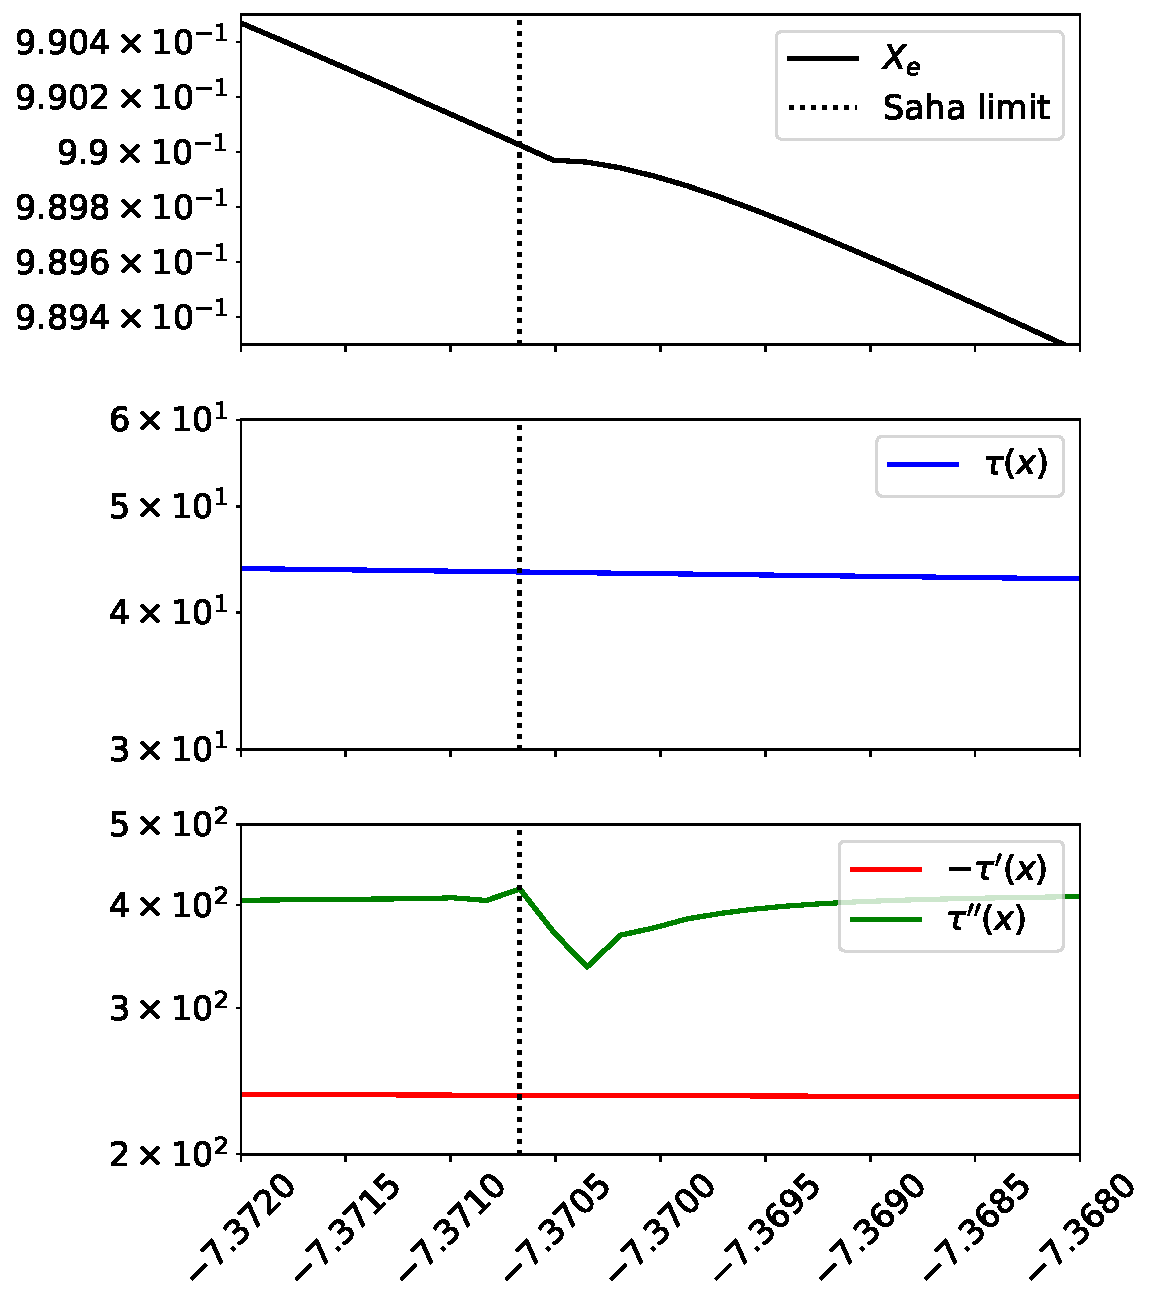
\includegraphics[scale=0.5]{../m2_figs/num_stab.pdf}
    \caption{Figure showing extremely zoomed in plots of $X_e$ as well as $\tau$ and its derivatives, around the transition point between the Saha and Peebles equations.}
    \label{fig:num_stab}
\end{figure}



\section{Electron number density} \label{sec:appendixC}
\begin{figure}[H]
    \centering
    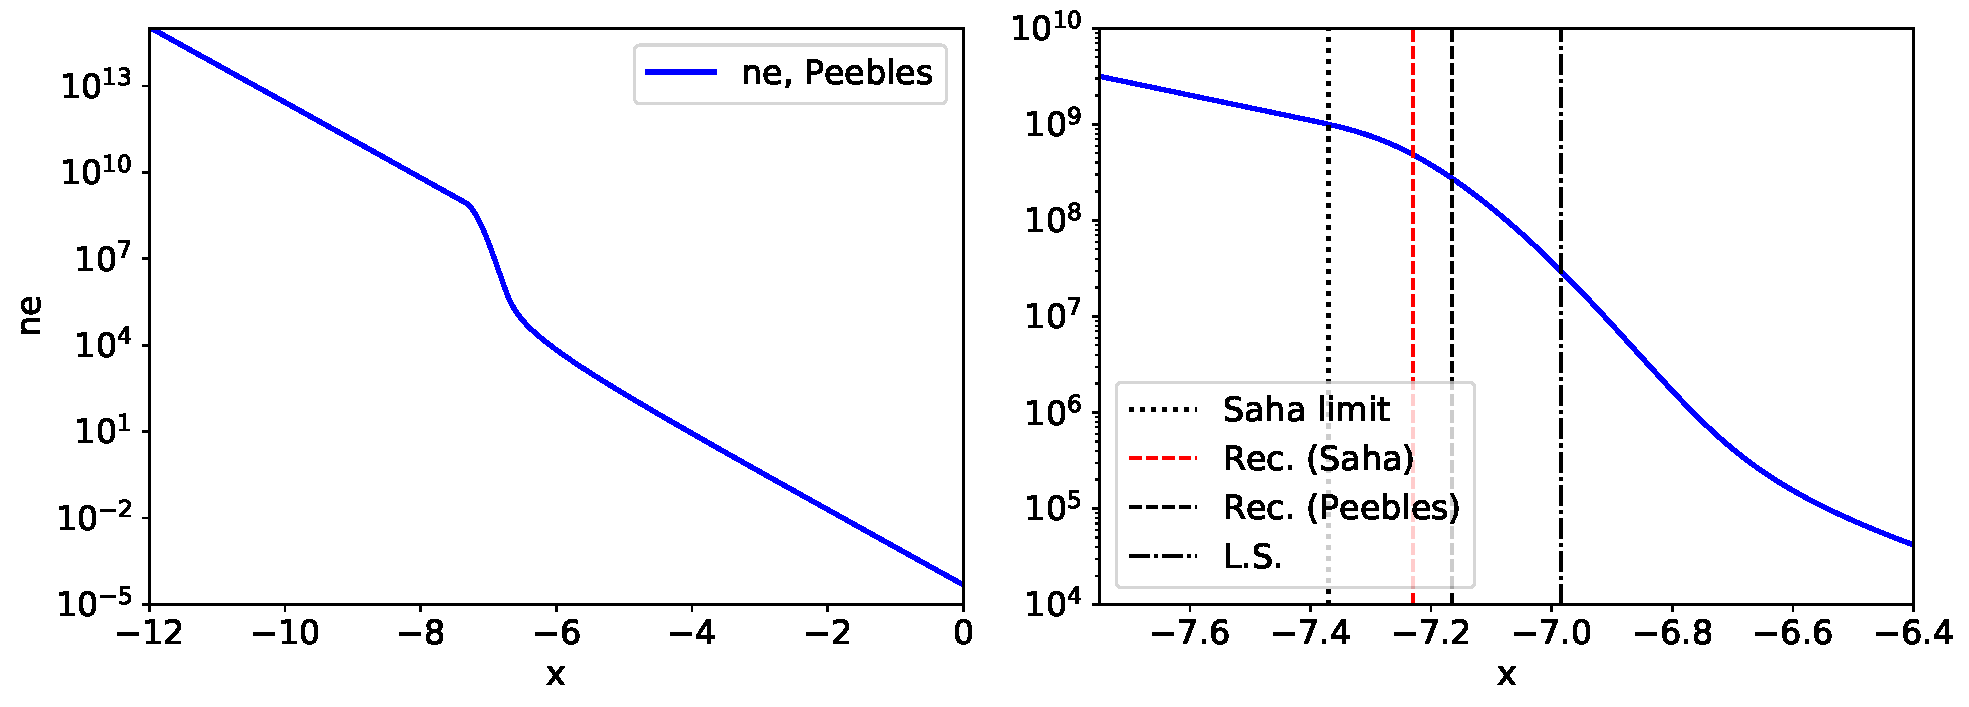
\includegraphics[scale=0.5]{../m2_figs/ne.pdf}
    \caption{}
    \label{}
\end{figure}


\bibliography{ref}
\bibliographystyle{plain}



\end{document}